\documentclass[11pt]{beamer}
\usepackage[utf8]{inputenc}
\usepackage[T1]{fontenc}
\usepackage{lmodern}

\usepackage{amsmath,amssymb}
\usepackage[shortlabels]{enumitem}
\usepackage{graphicx}

\title{Quasi-random number generator}
\author[Ines Meršak]{Ines Meršak \\
    Mentor: doc.~dr.~Dejan Velušček}
\date{21.~4.~2017}

\usetheme{Madrid}
\usecolortheme{beaver}

\begin{document}
\begin{frame}
    \maketitle
\end{frame}

\begin{frame}{Pseudo-random vs.~quasi-random}
    \alert{Pseudo-random number} 
    \begin{itemize}
        \item computer-generated number
        \item appears to be random
        \item generated by an entirely deterministic process
    \end{itemize}

    \bigskip
    
    \bigskip
    
    \alert{Quasi-random number}
    \begin{itemize}
        \item low-discrepancy number
        \item taking previous draws into account
    \end{itemize}
\end{frame}

\begin{frame}
    \begin{figure}
        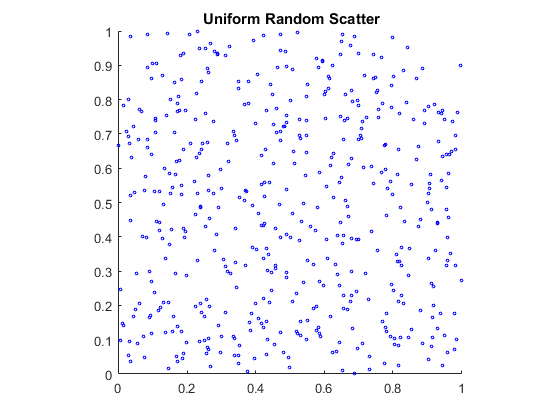
\includegraphics[width=180pt]{pseudo.png}
        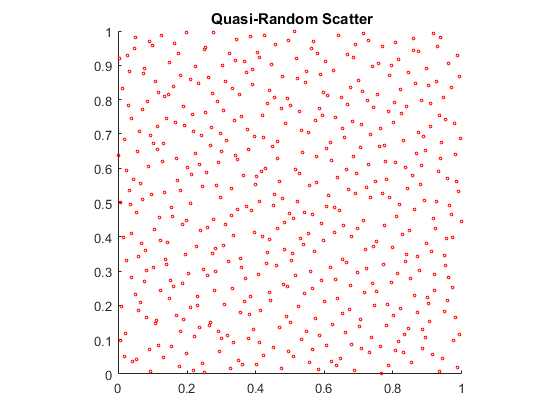
\includegraphics[width=180pt]{quasi.png}
    \caption{The comparison between pseudo- (left) and quasi-random numbers. (Source: \url{www.mathworks.com}.)}
    \end{figure}
\end{frame}

\begin{frame}{Usage}
    \begin{itemize}[--]
        \item useful in computational problems
        \medskip
        \item popular for financial Monte Carlo calculations 
        \medskip
        \item asymptotic convergence is faster than when using pseudo-random numbers
    \end{itemize}
\end{frame}

\begin{frame}{Sobol' numbers}
    \begin{itemize}[--]
        \item a new unique generating integer $\gamma(n)$ for each new draw 
        \item the generation is carried out on a set of integers in the interval $[1, 2^b-1]$
        \item $x_{nk}$ is the $n$th draw of Sobol' integer in dimension $k$
        \item a set of $b$ \alert{direction integers} for each dimension $k$
        \item for each dimension: select a primitive polynomial modulo two and calculate the direction integers using the coefficients of the polynomial and binary addition
        \item depending on which bits in the binary representation of $\gamma(n)$ are set, the direction integers are XORed to produce the Sobol' integer $x_{nk}$
    \end{itemize}
\end{frame}

\begin{frame}{Project timeline}
    Work done so far:
    \begin{itemize}[--]
        \item reading the source material
        \item getting familiar with C++
    \end{itemize}
    
    \bigskip
    
    Plan for the rest of the project: 
    \begin{itemize}[--]
        \item implement Sobol' number generator with Gray code (end of April)
        \item test the generator with quasi-Monte Carlo integration (first week of May)
        \item compare results with the parallel version (first week of May)
    \end{itemize}
\end{frame}

\end{document}